\documentclass{article}
\usepackage[version=3]{mhchem} % Package for chemical equation typesetting
\usepackage{siunitx} % Provides the \SI{}{} and \si{} command for typesetting SI units
\usepackage{graphicx} % Required for the inclusion of images
\usepackage{natbib} % Required to change bibliography style to APA
\usepackage{amsmath} % Required for some math elements 

\setlength\parindent{0pt} % Removes all indentation from paragraphs

\renewcommand{\labelenumi}{\alph{enumi}.} % Make numbering in the enumerate environment by letter rather than number (e.g. section 6)

\title{Détermination de g à l'aide \\ de la machine d'Atwood} % Title

\author{Collège \textsc{Sismondi}} 

\date{\today}

\begin{document}

\maketitle

\begin{center}
    \begin{tabular}{l r}
        Date de l'expréience: & Novembre 30, 2020 \\
        Expérimentateurs:     & Elena Gariglio    \\
                              & Noa Ette          \\
                              & Ozair Faizan      \\
        Professeur:           & Julien Ponard
    \end{tabular}
\end{center}


\section{But de l'expérience}

Déterminer la valeur de l'accélération gravitationnelle g des corps en chute libre à la surface de la Terre.


\section{Principe expérimental}
\label{definitions}
\begin{description}
    \item[La machine d'Atwood]
          est constituée d'une poulie pouvant tourner autour de son axe avec très peu de frottements. Des masses de valeurs très proches l'une de l'autre, reliées entre ellse par une ficelle de masse négligeable et inextensible passant par la poulie, peuvent être mises en mouvement sous l'effet de leur poids. En appliquand des petits forces à des masses grandes, la machine d'Atwood permet de réaliser des mouvements de chute à faible accélération, donc plus facilement mesurable. Puisque cette accélération dépend de g, il est ainsi possible de déduire simplement g en construisant le graphique des différences des masses en fonction de l'inverse du temos de chute au carré.
\end{description}


\section{Matériel et schéma de l'expérience}
\subsection{Matériel}
\begin{matériel_schéma}
Deux photocellules, horloge électonique et un jeu de masses pour crée la surcharge.

Les masses supports valent chaqu'un 70.0 g, les surcharges ont une masse globale de 16.00 g et la masse de la poulie est de 99.7 g.
\end{matériel_schéma}

\subsection{Schéma}


Figure \ref{fig:boat1}.

\section{Théorie de l'expérience}
\begin{enumerate}
    \begin{item}
        \begin{equation*}
        a = \frac{(m_{1} - m_{2})g}{m_{1} + m_{2} + \frac{M}{2}}
        \end{equation*}
    \end{item}
    \begin{item}
        \begin{equation*}
            g = \frac{2L(m_{1} + m_{2} + \frac{M}{2})}{(m_{1} - m_{2})({\Delta}t)^2}
        \end{equation*}
    \end{item}
    \begin{item}
          \begin{equation*} g = \frac{2LK}{pente}\end{equation*} \\ avec \\ \begin{equation*}K = m_{1} + m_{2} + \frac{M}{2}\end{equation*}
    \end{item}
\end{enumerate}


%----------------------------------------------------------------------------------------
%	SECTION 4
%----------------------------------------------------------------------------------------

\section{Results and Conclusions}

The atomic weight of magnesium is concluded to be \SI{24}{\gram\per\mol}, as determined by the stoichiometry of its chemical combination with oxygen. This result is in agreement with the accepted value.

\begin{figure}[h]
    \begin{center}
        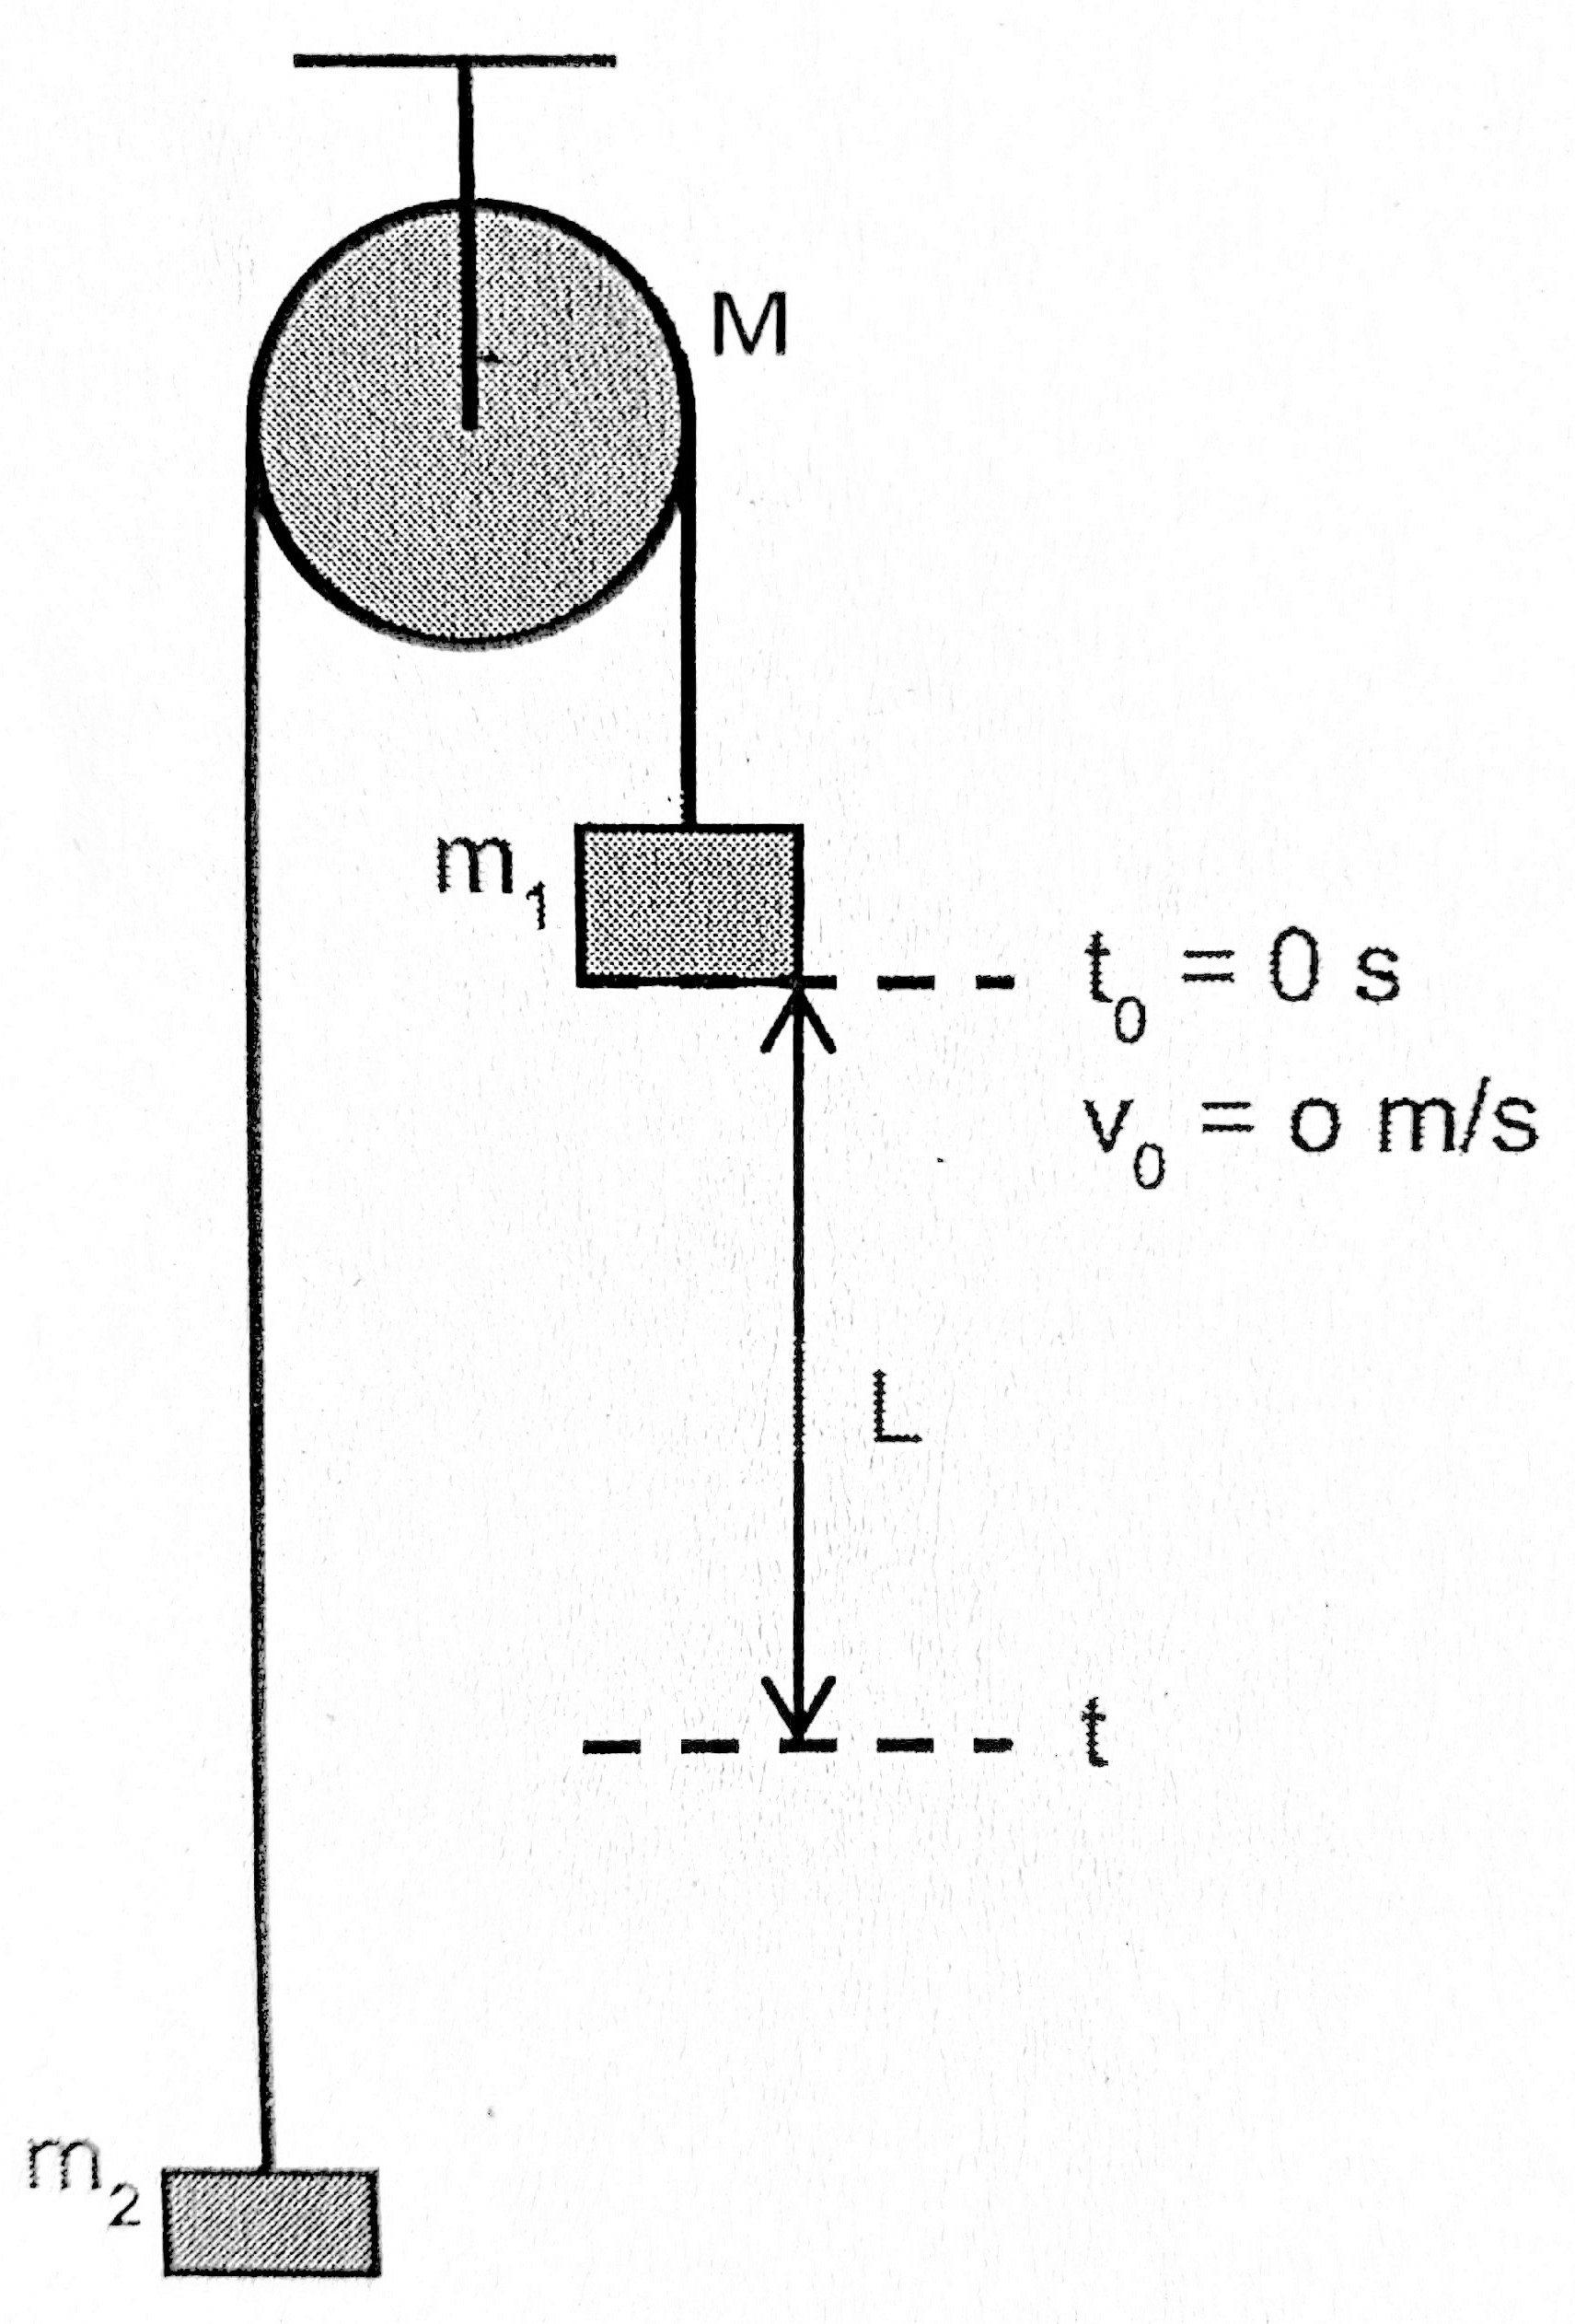
\includegraphics[width=0.65\textwidth]{okay.jpg} 
        \caption{Figure caption.}
    \end{center}
\end{figure}

%----------------------------------------------------------------------------------------
%	SECTION 5
%----------------------------------------------------------------------------------------

\section{Discussion of Experimental Uncertainty}

The accepted value (periodic table) is \SI{24.3}{\gram\per\mole} \cite{Smith:2012qr}. The percentage discrepancy between the accepted value and the result obtained here is 1.3\%. Because only a single measurement was made, it is not possible to calculate an estimated standard deviation.

The most obvious source of experimental uncertainty is the limited precision of the balance. Other potential sources of experimental uncertainty are: the reaction might not be complete; if not enough time was allowed for total oxidation, less than complete oxidation of the magnesium might have, in part, reacted with nitrogen in the air (incorrect reaction); the magnesium oxide might have absorbed water from the air, and thus weigh ``too much." Because the result obtained is close to the accepted value it is possible that some of these experimental uncertainties have fortuitously cancelled one another.


\section{Answers to Definitions}

\begin{enumerate}
    \begin{item}
          The \emph{atomic weight of an element} is the relative weight of one of its atoms compared to C-12 with a weight of 12.0000000$\ldots$, hydrogen with a weight of 1.008, to oxygen with a weight of 16.00. Atomic weight is also the average weight of all the atoms of that element as they occur in nature.
    \end{item}
    \begin{item}
          The \emph{units of atomic weight} are two-fold, with an identical numerical value. They are g/mole of atoms (or just g/mol) or amu/atom.
    \end{item}
    \begin{item}
          \emph{Percentage discrepancy} between an accepted (literature) value and an experimental value is
          \begin{equation*}
              \frac{\mathrm{experimental\;result} - \mathrm{accepted\;result}}{\mathrm{accepted\;result}}
          \end{equation*}
    \end{item}
\end{enumerate}

%----------------------------------------------------------------------------------------
%	BIBLIOGRAPHY
%----------------------------------------------------------------------------------------

\bibliographystyle{apalike}

\bibliography{sample}

%----------------------------------------------------------------------------------------


\end{document}